% Created 2020-10-01 Thu 19:37
% Intended LaTeX compiler: pdflatex
\documentclass[11pt]{article}
\usepackage[utf8]{inputenc}
\usepackage[T1]{fontenc}
\usepackage{graphicx}
\usepackage{grffile}
\usepackage{longtable}
\usepackage{wrapfig}
\usepackage{rotating}
\usepackage[normalem]{ulem}
\usepackage{amsmath}
\usepackage{textcomp}
\usepackage{amssymb}
\usepackage{capt-of}
\usepackage{hyperref}
\author{adam}
\date{\today}
\title{}
\hypersetup{
 pdfauthor={adam},
 pdftitle={},
 pdfkeywords={},
 pdfsubject={},
 pdfcreator={Emacs 26.3 (Org mode 9.3.8)}, 
 pdflang={English}}
\begin{document}

\tableofcontents

\section{Overview}
\label{sec:org8b8a77f}

\subsection{Course Structure}
\label{sec:orgd787973}
This course is an introduction to media theory – a subcategory of
philosophy that emerged in the mid 20th century as an attempt to
understand the impact that new technologies were having on the
individual and, in a broader sense, society. 
The general tone used to convey the ideas contained throughout the
notes and lectures will be an informal one, you refers to you the
reader, listener and student. We refers to the teachers, authors and 
students that have been consulted in developing the material for this 
course. Us refers to the group that we happen to find ourselves in at 
any particular moment in time. And I refers to me, the teacher, Adam McCartney.  
This course is intended to introduce undergraduate level music
students to the broader disciplines relevant for professional work in 
the arts and humanities. There are those who would consider it absurd 
that now, in the 21st century, investing in anything but a science
related degree is simply a waste. In the face of such beliefs, it is 
worth pausing briefly to remember a simple point made by John Henry
Newman, that a solid education in the liberal arts equips a student
with tools that will ultimately lead them to become better engineers, 
scientists, doctors, artists, lawyers and etc.   


\subsection{Philosophy of Teaching}
\label{sec:org3f86a85}
\begin{center}
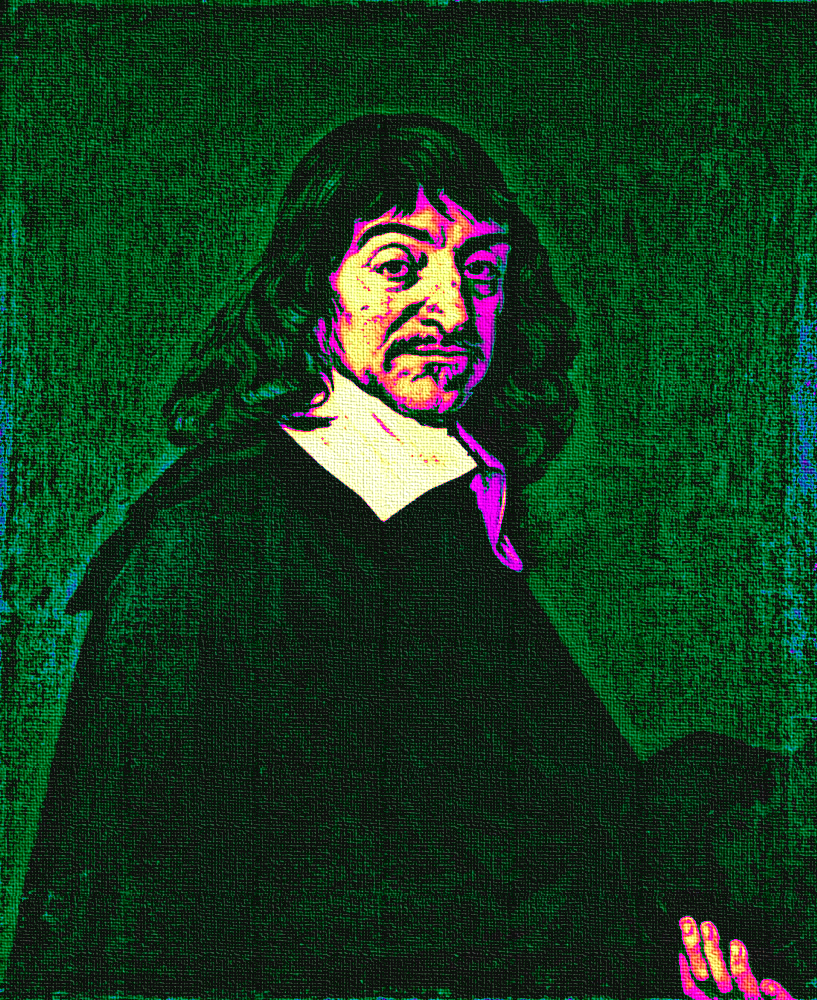
\includegraphics[width=.9\linewidth]{./descartes.png}
\end{center}
The satisfaction that can be gained through learning, teaching and
generally sharing information and can be immense. My more positive 
experiences over the years as a student and teacher have tended to 
come from courses, books, tutorials, videos, discussions that were 
clear enough to allow enable an understanding of the topic from 
first principles – that is to say that the material related to 
the topic was assembled in such a way as to reveal its most
fundamental ideas. Its virtually always beneficial to ask rudimentary 
questions about whatever it is that we are trying to understand, as 
such questions will quickly reveal whether or not the topic under 
discussion has a basis in fact. 
This course also aims to introduce some of the core methods that are
useful anywhere that it becomes necessary to think about something:

\begin{itemize}
\item Discourse
\item Reason
\item Logic
\item Debate
\item Reference
\end{itemize}


\subsubsection{7 Liberal Arts of the medieval university}
\label{sec:org3a6bc18}
\begin{itemize}
\item Grammar
\item Rhetoric
\item Logic
\item Geometry
\item Arithmetic
\item Music
\item Astronomy
\end{itemize}

\subsection{Where and how to access material}
\label{sec:org431f9b0}
The primary source of information for topics presented in this course
can be found in the VMI digital library, which is labelled \emph{Academic
Resources For Students} and will appear as a link on the homepage of
your Moodle eLearning profile. 
Please take the time to do the readings, this will prepare you for the
discussions that will take place during class. Thinking about things
is a practical exercise, it‘s the same as riding a bicycle or learning
to play an instrument. That means that the only way that you are going
to learn how to think is by engaging with the readings and
exercises. Much the same as any activity that is worth learning,
thinking is difficult and takes a lot of patience to get right. 
The texts that were chosen to be part of the course are all written in
an accessible style and are not overtly academic or
technical. Nevertheless, they do contain  ideas and arguments that you
might not get on the first reading.  My two favorite reading
disciplines  from when I was an undergraduate were the practice of
reading for a pre-allocated amount of time and also reading each text
at least three times in preparation for a class. 

\subsection{Portability and how to apply course content}
\label{sec:org69b1940}
Should you try and tell your piano tuner about Ludwig Wittgenstein‘s
ideas on the formation of knowledge? Definitely not! In fact, they
would be more likely to charge you extra fees just to get your piano
tuned if you chose to do so. 
So where exactly can this knowledge be applied? A friend of mine is a
hobby programmer and he recently told me his principle approach to
work. He called it „eat your own dogfood“. Now obviously the idea of
eating any kind of dogfood does not sound particularly appetizing, but
it is worth considering that dogs can also eat cake. The simple idea
here is that whatever type of idea or discipline you develop, it is
better first practiced on yourself before inflicting it upon the rest
of us; when properly cultivated a discipline is a way to nourish,
develop and sustain.




\section{The long 19th century (1789 - 1914)}
\label{sec:orgbd5b0d8}

\subsubsection{A brief history of art leading up to the industrial revolution}
\label{sec:org5b6c97f}
The renaissance had shown that the rise of merchant classes was
possible, and that there was room for a talented craftsperson to build
a career out of a good reputation. Still, even the most talented
artists from the renaissance and baroque periods werde subjects of
some royal court and often patronized (though less commonly so than in
the middle ages and early renaissance) by the clergy. The dominant
motives of these eras were, for instance, dedicated to the nobility
and to the church. An appreciation for human ingenuity was growing and
quietly, a new philosophy of reason and enlightenment was being born. 


\subsubsection{Art in the Age of Revolution (1789 - 1848)}
\label{sec:org0cb54d1}

Before it turned into a bloody mess, the core ideals of the French
Revolution (freedom, equality and brotherhood) seemed to be an
articulation of the broader hopes of humanity for a brighter future. 
Many of the artists of the late 18th and early 19th centuries echoed
these newly formed ideas of the enlightenment. 

\begin{itemize}
\item 50 years that included late Mozart, Haydn, Beethoven, Schubert, Goethe, Dickets,
Dostoievsky, Verdi, Wagner
\item Art made to appeal to a literate public that was increasing in
size
\item The invention of machinery reduced the cost of physical labor for
many, meaning there was more free time for education and pastimes
\item Aesthetic themes often contained pastoral elements, or sought to
simplify harmonies and form.
\item The influence from classical antiquity frequently appear, along with
references to similar threads from the renaissance
\end{itemize}

\begin{figure}[htbp]
\centering
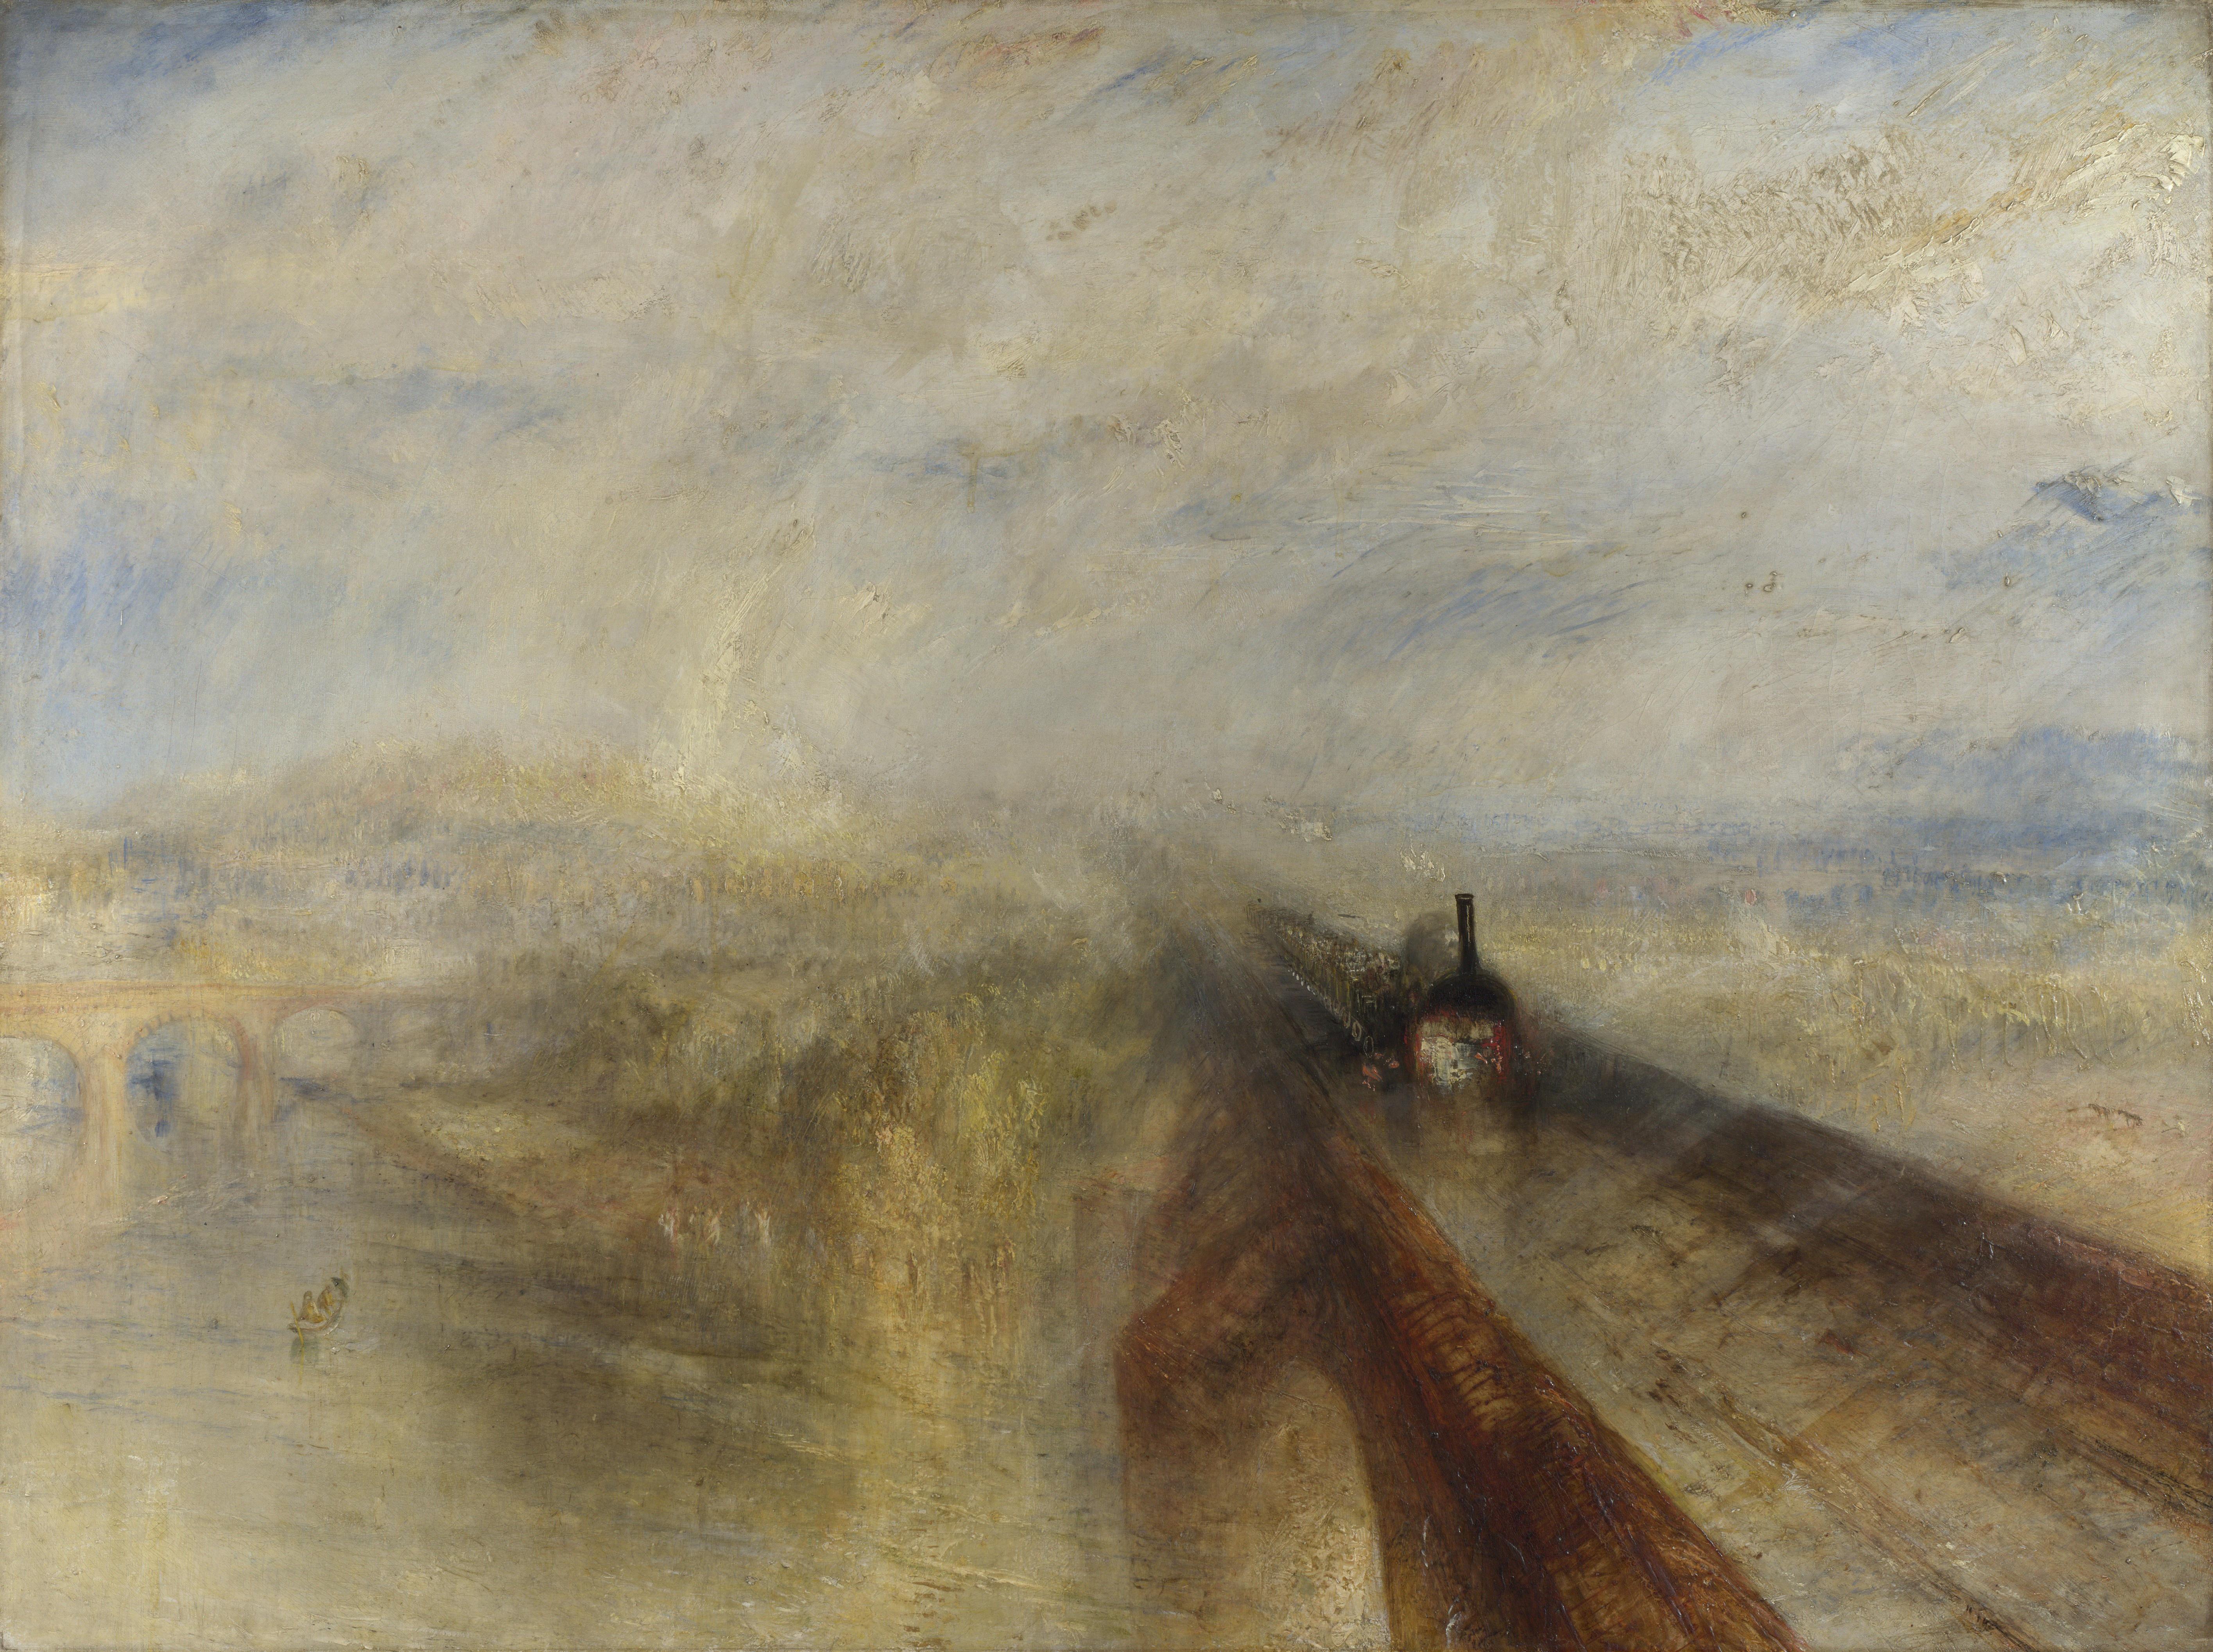
\includegraphics[width=.9\linewidth]{./Turner_-_Rain,_Steam_and_Speed_-_National_Gallery_file.jpg}
\caption{William Turner - Rain, Steam and Speed}
\end{figure} 

\subsubsection{Utopia}
\label{sec:org8451047}

Much of the art of the age focused utopian ideals, be they either in
some possible future or some glorified past: there were large
collections of folk tales, songs and verses that emerged during this
period that bore testiment to the vision of "the folk" as being
inherently virtuous. The new movements toward industrialized living
and a faster pace of life, on the other hand, was often viewed with at
least the usual amount of suspicion. Of course, the of a fall from
grace and the quest for redemption is literally as old as Adam and Eve.

\subsubsection{Art in the Age of Capital (1848 - 1875)}
\label{sec:org7fd21b6}

Having seen what the first half of the 19th century delivered in terms
of the arts, it's not surprising that this period during the later half of
the century appears somewhat underwhelming. Perhaps the real
achievements.
\begin{itemize}
\item the era produced a rather curious archictural style with
increasingly large proportions - this marks a contrast to the
classicaly influences in the styles (like Biedermeier) that
immediately preceded, where in central focus were human proportions
\item funding structures of the arts changed: they were now supported by
governments, bourgeoisie and incresingly the emerging working /
middle class
\item the viennese ring serves as a good example to the monuments of the age
\item first appearance of technically reproducable works of art (early
photo camera had an immediate and profound effect on painting
\item arts were in every sense popular by the third quarter of the
century, with widely distributed novels
\item possible for artists to earn a good living and many (even if not
rich) were well respected
\item arts came to occupy a semi-religious position for many of the new
middle class, also (in the case of the German speaking world) a
symbol of success and status to rival Britain's economic spoils
\item the artists were seen as sources of truth, authorities on beauty
\end{itemize}



\subsubsection{Art in the Age of Empire (1875 - 1914)}
\label{sec:org8483583}
Bourgeois identity crisis
\begin{itemize}
\item orientalism
\item pastiche
\end{itemize}

Established and entitled artistic circles 
\begin{itemize}
\item the Seccessions of Vienna \& Berlin
\item the New English Arts Club
\item successors to the French Impressionist Exhibition
\end{itemize}

The emergence of the avant-garde 
\begin{itemize}
\item very limited public reception
\item the anti-reality star? (like Picasso, appreciated for their
phenomenal output as opposed to the qualities or content of the work)
\end{itemize}

The birth of cinema


\subsection{The short 20th century (1914 - 1996): Art in the Age of Extremes}
\label{sec:orgf56506c}
\subsubsection{Features of the early 20th century art landscape}
\label{sec:orgbaf5c4f}

\begin{itemize}
\item Modernism
\item Dadaism, Constructivism, Surrealism
\item Decided move away from conventional Bourgeois tastes
\item Europe (Paris) between the wars
\item The invention of cinema \& jazz
\item Battleship Potemkin \{ watch?v=VMWMq4AEyjU \}
\item Jazz: syncopated afro rhythms meets mechanical reproduction
\item Murillo was out El Greco was in
\item Also rejected: Age of Capital and Age of Empire
\item Viennese Ring considered pompus \& inauthentic
\item most of the avant garde artists identified with progressive politics
\item rise of Hitler and Stalin meant that most of the avant garde immigrated to the USA
\item James Joyce Ulysses: going to the common man
\item Mass media and propaganda
\end{itemize}

\subsubsection{Postwar Arts}
\label{sec:orgf58a412}

\begin{itemize}
\item Rock \& Roll, the LP
\item the advertising industry
\item the emergence of pop art
\item Shift away from Europe
\item The establishment new social democratic norms post 1950 - massive increase government funding for the arts tax-breaks in the States for wealthy patrons
\item Art as Investment
\item Massive Expansion of higher education
\item Classical music - decline in old genres concealed by the enormous increase in their performance mostly a repertoire of dead classics
\item Personal Electronics
\end{itemize}


\section{Key works in the developoment of media theory}
\label{sec:org36ec788}
\subsection{Walther Benjamin: The Work of Art in the Age of Mechanical Reproduction}
\label{sec:org54b25d1}

\subsection{Marshall McCluhan: The Medium is the message}
\label{sec:orge02661b}
\url{https://web.mit.edu/allanmc/www/mcluhan.mediummessage.pdf}


\section{Hackers and the open source movement}
\label{sec:orge0a82cb}

\subsection{Eric Raymond}
\label{sec:org5e8997f}
\subsubsection{How to become a hacker}
\label{sec:org2ba5156}
\url{http://www.catb.org/esr/faqs/hacker-howto.html}
\subsubsection{The new hacker's dictionary}
\label{sec:org8a0a1ee}
\url{http://hackersdictionary.com/html/index.html}

\section{Navigating the digital world in the time of soul sucking mega corporations}
\label{sec:org07a9293}

\subsection{Douglas Rushkoff and Team Human}
\label{sec:org127db40}
\subsubsection{Program or be Programmed}
\label{sec:org50ccc62}
\url{https://www.youtube.com/watch?v=imV3pPIUy1k\&feature=youtu.be}

\subsubsection{Team Human Podcast}
\label{sec:orga913c9f}
\url{https://teamhuman.fm}

\section{A brief history of epistemology}
\label{sec:org815a1e6}
\subsection{A few short points on the formation of knowledge}
\label{sec:orga48e398}
\subsubsection{Ancient}
\label{sec:org81c5d2b}
\subsubsection{Early Modern}
\label{sec:org3e9b4d0}
\subsubsection{National States Period}
\label{sec:orgcbe66ab}
\subsubsection{Contemporary Perspectives}
\label{sec:org06f58d8}

\section{Adaptation and Adoption}
\label{sec:org2928f5d}
\subsection{Features of Intagibles}
\label{sec:org41eedd2}
\subsection{Shared Strategies – the automaton blues}
\label{sec:org0efd851}

\section{Course Work}
\label{sec:org898209f}
Semester requirements are to do the readings, and submit two essays,
one short (ca. 1000 words) and one longer (ca. 2500 words). Actually,
the medium that you present these works is flexible - in the past
students have produced podcasts, written essays, made lesson
plans. The important thing is that you work on forming an idea an
presenting it in a coherant way. 

\subsection{Where are the best places to borrow ideas?}
\label{sec:orgaa542e2}
\subsection{Can we please make music theory a little less boring?}
\label{sec:org91c9cf5}
\end{document}
